%
% File acl2018.tex
%
%% Based on the style files for ACL-2017, with some changes, which were, in turn,
%% Based on the style files for ACL-2015, with some improvements
%%  taken from the NAACL-2016 style
%% Based on the style files for ACL-2014, which were, in turn,
%% based on ACL-2013, ACL-2012, ACL-2011, ACL-2010, ACL-IJCNLP-2009,
%% EACL-2009, IJCNLP-2008...
%% Based on the style files for EACL 2006 by 
%%e.agirre@ehu.es or Sergi.Balari@uab.es
%% and that of ACL 08 by Joakim Nivre and Noah Smith

\documentclass[11pt,a4paper]{article}
\usepackage[hyperref]{acl2018}
\usepackage{times}
\usepackage{latexsym}
\usepackage{booktabs}
\usepackage[utf8]{inputenc}
\usepackage{hyperref}
\usepackage{graphicx}
\urlstyle{same}

% \usepackage{polski}


\aclfinalcopy % Uncomment this line for the final submission
%\def\aclpaperid{***} %  Enter the acl Paper ID here

%\setlength\titlebox{5cm}
% You can expand the titlebox if you need extra space
% to show all the authors. Please do not make the titlebox
% smaller than 5cm (the original size); we will check this
% in the camera-ready version and ask you to change it back.

\newcommand\BibTeX{B{\sc ib}\TeX}

\title{I want to buy a property! The Analysis of The Market in Poznan 2018}

\author{Tomasz Dwojak \\
  Adam Mickiewicz University \\
  {\tt t.dwojak@amu.edu.pl}
}

\date{}

\begin{document}
\maketitle
\begin{abstract}
  In this report, we analyse the housing market in Poznan using advertisements from a popular portal. We show what factors have an impact on the price. Moreover, we build a linear regression model to predict the price of the property.
\end{abstract}

\section{Introduction}
Buying a flat is one of the most important decision in life and the most expensive one. In most cases, it follows getting a mortgage and paying it off for the next ten, twenty or thirty years. Besides, saving 10\% of the flat cost could have a huge impact on the total cost of the transaction.


\subsection{Obtaining data}
The data comes from a well-known portal \url{https://www.gratka.pl}, which allows for crawling data\footnote{See \url{https://gratka.pl/robots.txt}}. We use a simple Python script to download advertisements from Poznan: we use \emph{requests} library for accessing online data and \emph{Beautiful Soup} for parsing HTML. The data comes from February 2018.


\subsection{General Information}
The dataset contains in total 7383 offers of selling flats, houses and other properties like business premises. Table \ref{table:2018_features} contains a list of features and how often they repeated in the offers. In total, there are 39 features, but no offer has information about all of them. The only required feature is the price. However, some sellers set the cost of the property to zero (130 offers), and the next 190 set the price to less than 10,000 PLN. We treat those examples as an unlabelled data. Figure\ref{fig:features} shows the number of advertisements by given number of features. An offer has from 5 to 23 features with the average 12.43 and standard derivation of 3.28. Also, we collected text description and link to offers. Table  \ref{table:2018_features} contains the list of features and how many times they occur in the data set. Clearly, some features are closely related to the particular type of a property, e.g.\ roof type, having attic and area shape.
\begin{figure}[htpb]
  \centering
  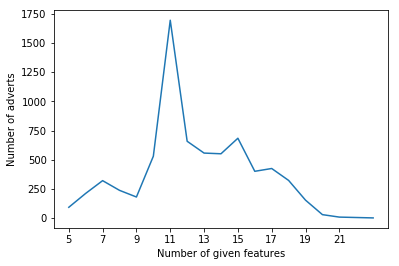
\includegraphics[width=0.8\linewidth]{./plots/features.png}
  \caption{Number of given features.}\label{fig:features}
\end{figure}


\begin{table}[ht]
  \centering
  \caption{Feature counts in data set 2018. The values are sorted decently.}\label{table:2018_features}
  \begin{tabular}{lr}
    \toprule
    Feature &     Counts \\
    \midrule
    Expected                         &  7383 \\
    URL                              &  7383 \\
    Description                      &  7383 \\
    Area                             &  6635 \\
    Parking Spot                     &  6607 \\
    Rooms                            &  6203 \\
    Number of floors in the building &  6138 \\
    Floor                            &  5557 \\
    Type                             &  4877 \\
    Window Type                      &  3744 \\
    Building Material                &  2666 \\
    Building Year                    &  2627 \\
    Ownership Type                   &  2552 \\
    Kitchen Type                     &  1976 \\
    Condition                        &  1506 \\
    Instalation Condition            &  1272 \\
    Noisiness                        &  1202 \\
    Access Road                      &   983 \\
    Bathroom Condition               &   968 \\
    Total Surface Area               &   745 \\
    Investition Name                 &   610 \\
    Area Shape                       &   572 \\
    Roof                             &   481 \\
    Sewage System                    &   427 \\
    Fence Type                       &   392 \\
    Basement                         &   388 \\
    Attic                            &   160 \\
    Elevation                        &   159 \\
    Type of Room                     &   158 \\
    Has Bathroom                     &    47 \\
    Available Time                   &    39 \\
    Number of Parking Spots          &    10 \\
    Electricity                      &     5 \\
    Gas                              &     3 \\
    Usable Area                      &     3 \\
    Water                            &     3 \\
    Parking Slots2                   &     2 \\
    Construction                     &     2 \\
    Number of Spaces                 &     1 \\
    \bottomrule
  \end{tabular}
\end{table}

\subsection{Getting data from URL}
We noticed that the URL structure is informative and contains data about the type of property and the localization. Appparently, the dataset includes the feature \emph{Type} but it is not complete. We use the three most popular forms of properties: flat, house, and business premises. The rest of offers have a common class entitled \emph{other}, which contains mainly garages and building lands. 



\begin{figure}[htpb]
  \centering
  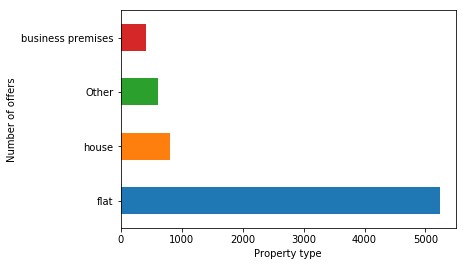
\includegraphics[width=0.8\linewidth]{./plots/proporty_types_h.png}
  \caption{Offers by property types.}
  \label{fig:property_types}
\end{figure}

The second feature we get from the URL is localization, which we limited to the extraction of 26 distinct names.
\begin{figure}[htpb]
  \centering
  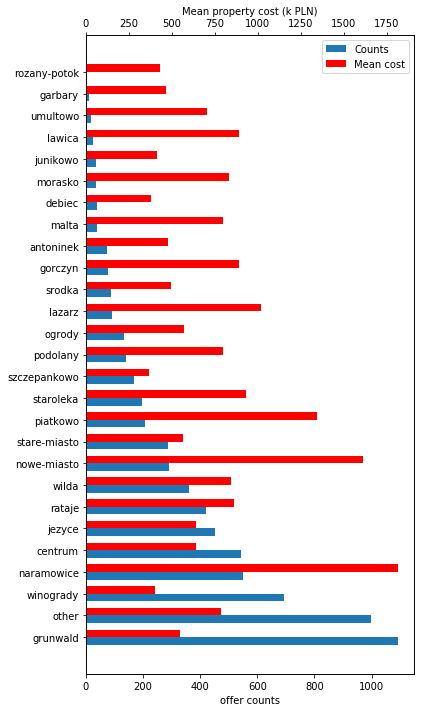
\includegraphics[width=0.8\linewidth]{./plots/distincts.png}
  \caption{Offers by distincts.}\label{fig:dist}
\end{figure}
\subsection{Data Preprocessing}%
\label{sub:preprocessing}
We performed a necessery data preprocessing. We transformed the values from the \emph{Expected} column to numerical form by removing spaces and changing colons to dots due to English notation system.

The column \emph{Rooms} contains the text ``more than 8 rooms'', which we replaced to a value of 9.

\section{The Market Analysis}
The average price of a property in Poznan in 2018 is 676320.12 PLN. The average cost depends on the property type. Figure \ref{fig:cost} shows the average property price by the type of the property. We see that flats and houses are much cheaper than properties for business. The average price for a flat is 373,293 PLN and 981,466 PLN for a house.
\begin{figure}[htpb]
  \centering
  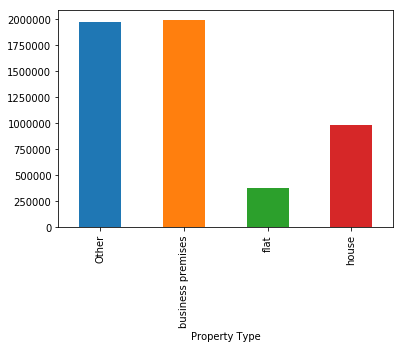
\includegraphics[width=0.8\linewidth]{./plots/prop_costs.png}
  \caption{Average cost by property type.}
  \label{fig:cost}
\end{figure}

Figure~\ref{fig:dist} shows the number of offers and the average cost in each distinct. The most expensive area is \emph{Naramowice} with the average exceeding 1,000,000 PLN.
The second place is for \emph{Nowe Miasto}, which is the old name for the north part of Poznan.

The most popular area is \emph{Grunwald} distinct with more than 1,000 offers: 117 house offer and 852 flat offers.


\section{House and Flat Price Prediction}
In this section, we describe models for predicting the price of houses and flats, which is the most common case with 6034 examples. Furthermore, we removed three offers with no given area. 

\subsection{Feature Selection}%
\label{sub:feature_selection}
Firstly, we reduced the feature set to features with at least 1000 occurances in the flat \& house data set. Finally, we decided to keep the following features: \emph{Area}, \emph{Rooms}, \emph{Localization} and \emph{Type}. For the last two features, we replaced them with dummies variables.

\subsection{Baseline Models}%
\label{sub:baseline_models}
We chose RMSE as a metric for this task and splitted the dataset to train-set (80\%) and (20\%) We build two baseline models basing on the mean of prices. The first model returns the mean of training data and the second one: the mean by property types. We see that the second model performs much better than the first one.
\begin{table}[]
  \centering
  \caption{Model scores}
  \label{my-label}
  \begin{tabular}{|l|l|}
    \hline
    Model                        & RMSE                           \\ \hline
    Baseline: mean               & \multicolumn{1}{r|}{509858.69} \\ \hline
    Baseline: mean by type       & 449749.60                      \\ \hline
    Linear Regression            & 388061.35                      \\ \hline
    Linear Regression (Area)     & 432959.30                      \\ \hline
    Lasso                        & 388063.85                      \\ \hline
    Ridge                        & 388102.25                      \\ \hline
    ElasticNet                   & 396977.63                      \\ \hline
    kNN-5                        & 354513.54                      \\ \hline
    kNN-1                        & 332836.70                      \\ \hline
    SVM                          & 355171.41                      \\ \hline
  \end{tabular}
\end{table}

\subsection{Linear Regression}%
\label{sub:linear_regression}
We started with simple linear regression model. First, we trained a model on the whole feature set. Later, we experimented with regularization. We figure out that only $L_2$ penalty helps, but not much.

Lately, we trained model for each feature separately. The lowest result was obtained for the \emph{Area}. Moreover, model based on location information only perform a slightly better than the first baseline.
Low scores obtained by linear regression models may sugest about non-linear dependency between features and the flat price.
\subsection{KNN}%
\label{sub:knn}
Nextly, we train nonlinear regressors. We started with with $k$ Nearest Neighbors. To our suprise, the knn-1 model outperforms linear regression and achieved the lowest RMSE.


\section*{Conclusion}
In this report we described the data about property market in Poznan. We showed, that the most popular properties are flats on the West part of the city. Also, we tested different regressors for prediction of the property price, which seems to be a challange due to nonlinear dependencies.

% include your own bib file like this:
%\bibliographystyle{acl}
%\bibliography{acl2018}
%\bibliography{acl2018}
%\bibliographystyle{acl_natbib}


\end{document}
